\documentclass[11pt]{article}

\usepackage{float}
\usepackage{hyperref}
\usepackage{graphicx}
% formatting
\usepackage{verbatim}
\usepackage{moreverb}
\usepackage{minted}
\usepackage{parskip}
\usepackage{amsmath}
\usepackage[listings]{tcolorbox}
\usepackage{enumerate}
\let\verbatiminput=\verbatimtabinput
\def\verbatimtabsize{4\relax}

\newcommand{\RepoRootPath}{fpga\_labs\_fa19}

\tcbset{
texexp/.style={colframe=black, colback=lightgray!15,
         coltitle=white,
         fonttitle=\small\sffamily\bfseries, fontupper=\small, fontlower=\small},
     example/.style 2 args={texexp,
title={Question \thetcbcounter: #1},label={#2}},
}

\newtcolorbox{texexp}[1]{texexp}
\newtcolorbox[auto counter]{texexptitled}[3][]{%
example={#2}{#3},#1}

\setlength{\topmargin}{-0.5in}
\setlength{\textheight}{9in}
\setlength{\oddsidemargin}{0in}
\setlength{\evensidemargin}{0in}
\setlength{\textwidth}{6.5in}

% Useful macros

\newcommand{\note}[1]{{\bf [ NOTE: #1 ]}}
\newcommand{\fixme}[1]{{\bf [ FIXME: #1 ]}}
\newcommand{\wunits}[2]{\mbox{#1\,#2}}
\newcommand{\um}{\mbox{$\mu$m}}
\newcommand{\xum}[1]{\wunits{#1}{\um}}
\newcommand{\by}[2]{\mbox{#1$\times$#2}}
\newcommand{\byby}[3]{\mbox{#1$\times$#2$\times$#3}}


\newenvironment{tightlist}
{\begin{itemize}
 \setlength{\parsep}{0pt}
 \setlength{\itemsep}{-2pt}}
{\end{itemize}}

\newenvironment{titledtightlist}[1]
{\noindent
 ~~\textbf{#1}
 \begin{itemize}
 \setlength{\parsep}{0pt}
 \setlength{\itemsep}{-2pt}}
{\end{itemize}}

% Change spacing before and after section headers

\makeatletter
\renewcommand{\section}
{\@startsection {section}{1}{0pt}
 {-2ex}
 {1ex}
 {\bfseries\Large}}
\makeatother

\makeatletter
\renewcommand{\subsection}
{\@startsection {subsection}{1}{0pt}
 {-1ex}
 {0.5ex}
 {\bfseries\normalsize}}
\makeatother

% Reduce likelihood of a single line at the top/bottom of page

\clubpenalty=2000
\widowpenalty=2000

% Other commands and parameters

\pagestyle{myheadings}
\setlength{\parindent}{0in}
\setlength{\parskip}{10pt}

% Commands for register format figures.

\newcommand{\instbit}[1]{\mbox{\scriptsize #1}}
\newcommand{\instbitrange}[2]{\instbit{#1} \hfill \instbit{#2}}

\begin{document}

\def\PYZsq{\textquotesingle}
\title{\vspace{-0.4in}\Large \bf EECS 151/251A FPGA Lab 3:\\Tone Generator, Simulation, and Connecting Modules\vspace{-0.1in}}

\author{Prof. Borivoje Nikolic and Prof. Sophia Shao \\
TAs: Cem Yalcin, Rebekah Zhao, Ryan Kaveh, Vighnesh Iyer \\ Department of Electrical Engineering and Computer Sciences\\
College of Engineering, University of California, Berkeley}
\date{}
\maketitle

\newcommand{\headertext}{EECS 151/251A FPGA Lab 3: Simulation and Sequential Circuits}
\markboth{\headertext}{\headertext}
\thispagestyle{empty}

\section{Before You Start This Lab}
Before you proceed with the contents of this lab, we suggest that you look through these two documents that will help you better understand some Verilog constructs.

\begin{enumerate}
  \item \href{http://inst.eecs.berkeley.edu/~eecs151/fa19/files/verilog/wire_vs_reg.pdf}{wire\_vs\_reg.pdf} - The differences between wire and reg nets and when to use each of them.
  \item \href{http://inst.eecs.berkeley.edu/~eecs151/fa19/files/verilog/always_at_blocks.pdf}{always\_at\_blocks.pdf} - Understanding the differences between the two types of always @ blocks and what they synthesize to.
\end{enumerate}

\subsection{Running the Lab on Your Laptop}
If you want to run the tools for this lab locally, refer to the appendix.

\section{Designing a Tone Generator}
Let's create a tone generator/buzzer on the FPGA.

\subsection{Clock Sources}
Look at the \href{https://reference.digilentinc.com/reference/programmable-logic/pynq-z1/reference-manual}{Pynq Reference Manual}.
Read Section 11 about the clock sources available on the Pynq.
We are using the 125 MHz clock from the Ethernet PHY IC on the Pynq board connected to pin H12 of the FPGA chip.

Look at the \texttt{src/z1top.v} top-level module and its \verb|CLK_125MHZ_FPGA| input.
\begin{minted}{verilog}
module z1top (
    input CLK_125MHZ_FPGA,
    ...
);
\end{minted}
Next take a look at the constraints in \texttt{src/PYNQ-Z1\_C.xdc} and notice how the LOC for the clock net is set to H16, just as specified in the Pynq-Z1 Reference Manual.
\begin{minted}{tcl}
set_property -dict { PACKAGE_PIN H16 IOSTANDARD LVCMOS33 } \
  [get_ports { CLK_125MHZ_FPGA }];
\end{minted}
This is how we map top-level signals in Verilog to the physical FPGA pins they are connected to.
We can access the clock signal from our Verilog top-level module and can propagate this clock signal to any submodules that may need it.

\subsection{Audio Out}
Look at Section 14 of the \href{https://reference.digilentinc.com/reference/programmable-logic/pynq-z1/reference-manual}{Pynq Reference Manual} which describes the mono audio out feature on the Pynq board.

The FPGA pin R18 is connected to the \verb|AUD_PWM| net.
The FPGA can drive this net with a PWM signal which goes through a low-pass filter and is driven into the audio jack on the Pynq board.

There's also an \verb|AUD_SD| net connected to FPGA pin T17, which turns off the opamps in the low-pass filter.
Setting \verb|AUD_SD| to 1 enables the audio output.

Find these signals in the \texttt{src/PYNQ-Z1\_C.xdc} file, and note how they appear in the \texttt{src/z1top.v} port list.

\subsection{Generating a Square Wave}
Let's play a 220 Hz square wave out of the Mono Audio Out port on the Pynq.
The square wave should have a 50\% duty cycle, so for half of the period of one wave the signal should be high and for the other half, the signal should be low.
We have a 125 MHz clock we can use to time our circuit.

Find the following:
\begin{texexptitled}{Square Wave Calculations}{}
\begin{enumerate}[a)]
\item The period of our clock signal (frequency = 125 MHz)?
\item The period of a 220 Hz square wave?
\item How many clock cycles fit in one period of the square wave?
\end{enumerate}
\end{texexptitled}

Open \verb|src/tone_generator.v| and design a circuit to output a 220Hz square wave on the \verb|square_wave_out| output.
Ignore the \verb|tone_switch_period|, \verb|output_enable|, and \verb|volume| inputs for now.

\section{Simulating the Tone Generator}
Let's run some simulations on the \verb|tone_generator| in software to check it works before putting it on the FPGA.
To do this, we will need to use a Verilog testbench.
A Verilog testbench is designed to test a Verilog module by supplying it with the inputs it needs (stimulus signals) and testing whether the outputs of the module match what we expect.

\subsection{Overview of Testbench Skeleton}
Check the provided testbench skeleton in \verb|sim/tone_generator_testbench.v|.
Let's go through what every line of this testbench does.

\begin{minted}{verilog}
`timescale 1ns/1ns
\end{minted}

The timescale declaration needs to be at the top of every testbench file.
\begin{minted}{verilog}
`timescale (simulation step time)/(simulation resolution)
\end{minted}

The first argument to the timescale declaration is the simulation step time.
It defines the granularity of discrete time units in which the simulation advances.
In this case, we have defined the simulation step time to be one nanosecond, so we can advance the simulation time by as little as 1ns at a time.

The second argument to the timescale declaration is the simulation resolution.
In our example it is also 1ns.
The resolution allows the simulator to model transient behavior of your circuit in between simulation time steps.
For this lab, we aren't modeling any gate delays, so the resolution can safely equal the step time.

\begin{minted}{verilog}
`define SECOND 1000000000
`define MS 1000000
// The SAMPLE_PERIOD corresponds to a 44.1 kHz sampling rate
`define SAMPLE_PERIOD 22675.7
\end{minted}

These are some macros defined for our testbench.
They are constant values you can use when writing your testbench to simplify your code and make it obvious what certain numbers mean.
For example, \verb|SECOND| is defined as the number of nanoseconds in one second.
The \verb|SAMPLE_PERIOD| is the sampling period used to sample the square wave output of the \verb|tone_generator| at a standard 44.1 kHz sample rate.

\begin{minted}[tabsize=4]{verilog}
module tone_generator_testbench();
  // Testbench code goes here
endmodule
\end{minted}

\verb|tone_generator_testbench| is a testbench module.
It is not intended to be placed on an FPGA, but rather it is to be run by a circuit simulator.
All your testbench code goes in this module.
We will instantiate our DUT (device under test) in this module.

\begin{minted}{verilog}
reg clock;
reg output_enable;
reg volume = 0;
reg [23:0] tone_to_play;
wire sq_wave;
\end{minted}

Here are the inputs and outputs of our \verb|tone_generator|.
Notice that the inputs to the \verb|tone_generator| are declared as \verb|reg| type nets and the outputs are declared as \verb|wire| type nets.
This is because we will be driving the inputs in our testbench inside an \verb|initial| block and we will be reading the output.
Note we can set the initial value of \verb|reg| nets in the testbench to drive a particular value into the DUT at time 0 (e.g. \verb|volume|).

\begin{minted}{verilog}
initial clock = 0;
always #(4) clock <= ~clock;
\end{minted}

This is the clock generation code.
The clock signal needs to be generated in our testbench so it can be fed to the DUT.
The initial statement sets the value of the clock net to 0 at the very start of the simulation.
The next line toggles the clock signal every 4ns, i.e. half period of 125 MHz clock.

\begin{minted}[tabsize=4]{verilog}
tone_generator audio_controller (
    .clk(clock),
    .output_enable(output_enable),
    .tone_switch_period(tone_to_play),
    .volume(volume),
    .square_wave_out(sq_wave)
);
\end{minted}

Now we instantiate the DUT and connect its ports to the nets we have declared in our testbench.

\begin{minted}[tabsize=4]{verilog}
initial begin
    tone_to_play = 24'd0;
    output_enable = 1'b0;
    #(10 * `MS);
    output_enable = 1'b1;

    tone_to_play = 24'd37500;
    #(200 * `MS);
    ...
    $finish();
end
\end{minted}

This is the body of our testbench.
The \verb|initial begin ... end| block is the `main()' function for our testbench, and where the simulation begins execution.
In the \verb|initial| block we drive the DUT inputs using blocking (\verb|=|) assignments.

We can also order the simulator to advance simulation time using delay statements.
A delay statement takes the form \verb|#(delay in time steps);|.
For instance the statement \verb|#(100);| would run the simulation for 100ns.

In this case, we set \verb|output_enable| to 0 at the start of the simulation, let the simulation run for 10ms, then set \verb|output_enable| to 1.
Then \verb|tone_to_play| is changed several times, and the \verb|tone_generator| is given some time to produce the various tones.

The final statement is a system function: the \verb|$finish()| function tells the simulator to halt the simulation.

\begin{minted}[tabsize=4]{verilog}
integer file;
initial begin
  file = $fopen("output.txt", "w");
  forever begin
    $fwrite(file, "%h\n", sq_wave);
    #(`SAMPLE_PERIOD);
  end
end
\end{minted}

This piece of code is written in a separate \verb|initial begin ... end| block.
The simulator treats both \verb|initial| blocks as separate threads that both start execution at the beginning of the simulation and run in parallel.

This block of code uses two system functions \verb|$fopen()| and \verb|$fwrite()|, that allow us to write to a file.
The \verb|forever begin| construct tells the simulator to run the chunk of code inside it continuously until the simulation ends.

In the \verb|forever begin| block, we sample the \verb|square_wave_out| output of the \verb|tone_generator| and save it in \verb|output.txt|.
We sample this value every \verb|`SAMPLE_PERIOD| nanoseconds which corresponds to a 44.1 kHz sampling rate.
The \verb|tone_generator|'s output is stored as 1s and 0s in \verb|output.txt| that can be converted to an audio file to hear how your circuit will sound when deployed on the FPGA.

\subsection{Running the Simulation}
There are 2 RTL simulators we can use:
\begin{itemize}
  \item \textbf{VCS} - proprietary, only available on lab machines, fast
  %\item \textbf{XSIM} - free, bundled with Vivado, somewhat slower
  \item \textbf{Icarus Verilog} - open source, runs on Windows/OSX/Linux, somewhat slower
\end{itemize}
They all take in Verilog RTL and a Verilog testbench module and output:
\begin{itemize}
  \item A waveform file (.vpd, .vcd) that plots each signal in the testbench and DUT across time
  \item A text dump containing anything that was printed during the testbench execution
\end{itemize}

\subsubsection{VCS}
If you're using the lab machines, you should use VCS:
\begin{minted}{bash}
  make sim/tone_generator_testbench.vpd
\end{minted}
This will generate a waveform file \verb|sim/tone_generator_testbench.vpd| which you can view using \verb|dve|.
Login to the lab machines physically or use X2go and run:
\begin{minted}{bash}
  dve sim/tone_generator_testbench.vpd &
\end{minted}

The DVE interface contains 3 panels (Figure \ref{fig:dve}).
\begin{figure}[h]
  \centering
  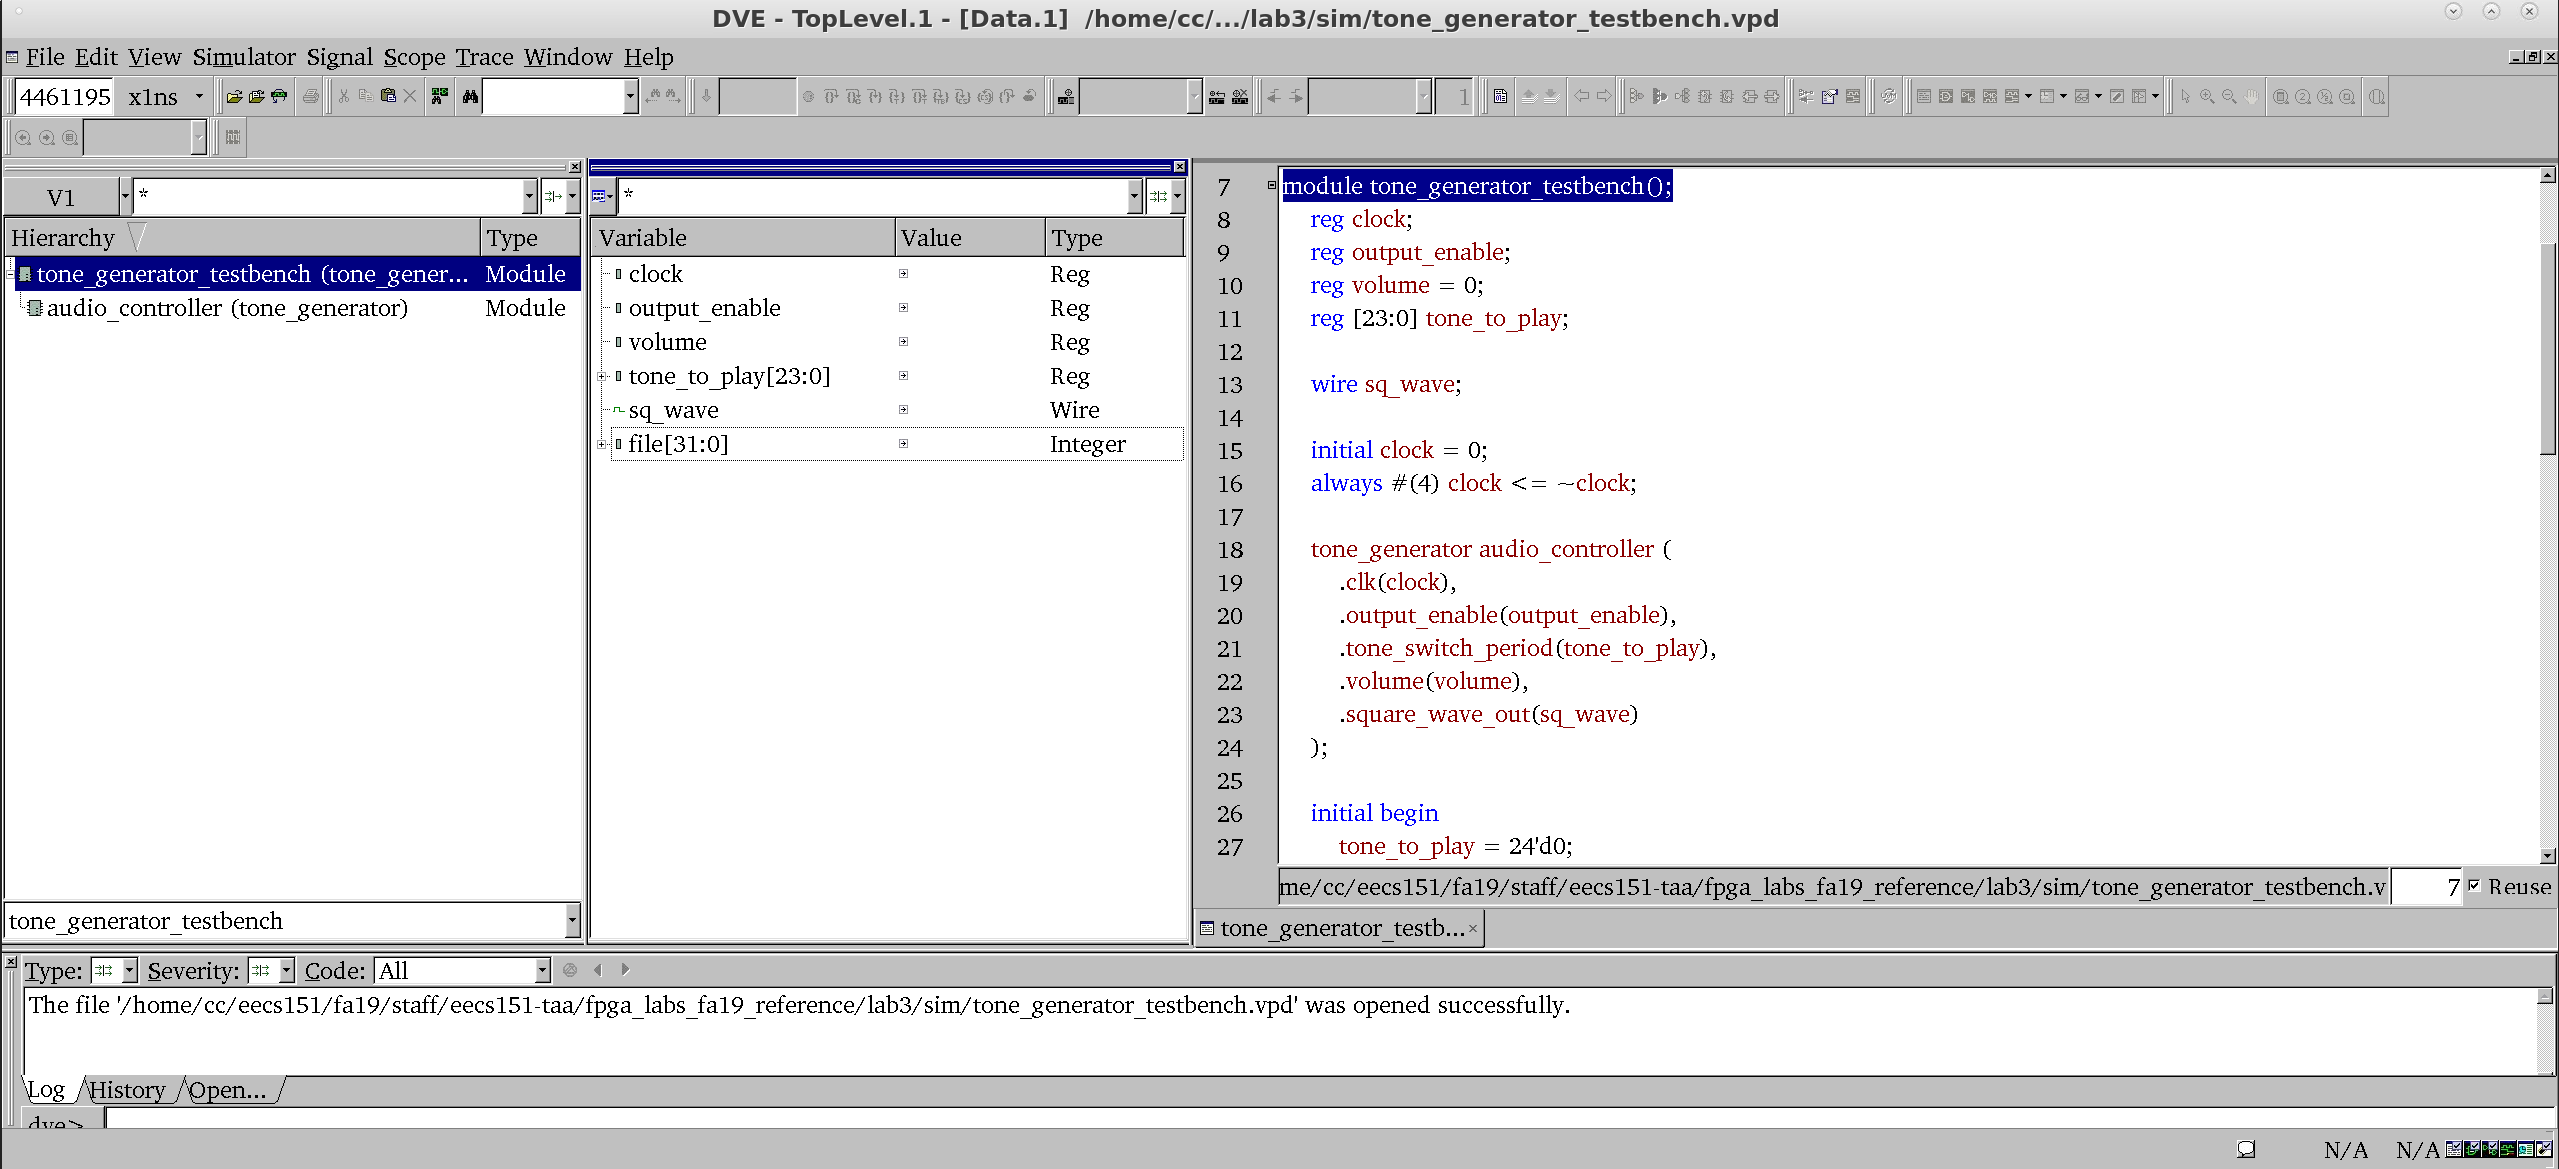
\includegraphics[width=\textwidth]{figs/dve.png}
  \caption{DVE Interface}
  \label{fig:dve}
\end{figure}

From left to right, you can see the `Hierarchy', `Signals', and `Source Code' windows.
The `Hierarchy' window lets you select a particular module instance in the testbench to view its signals.
In the `Signals' window, you can select multiple signals (by Shift-clicking) and then right-click $\rightarrow$ `Add To Waves' $\rightarrow$ `New Wave View' to plot the waveforms for the selected signals.

The waveform viewer is shown in Figure \ref{fig:dve_wave}.
\begin{figure}[h]
  \centering
  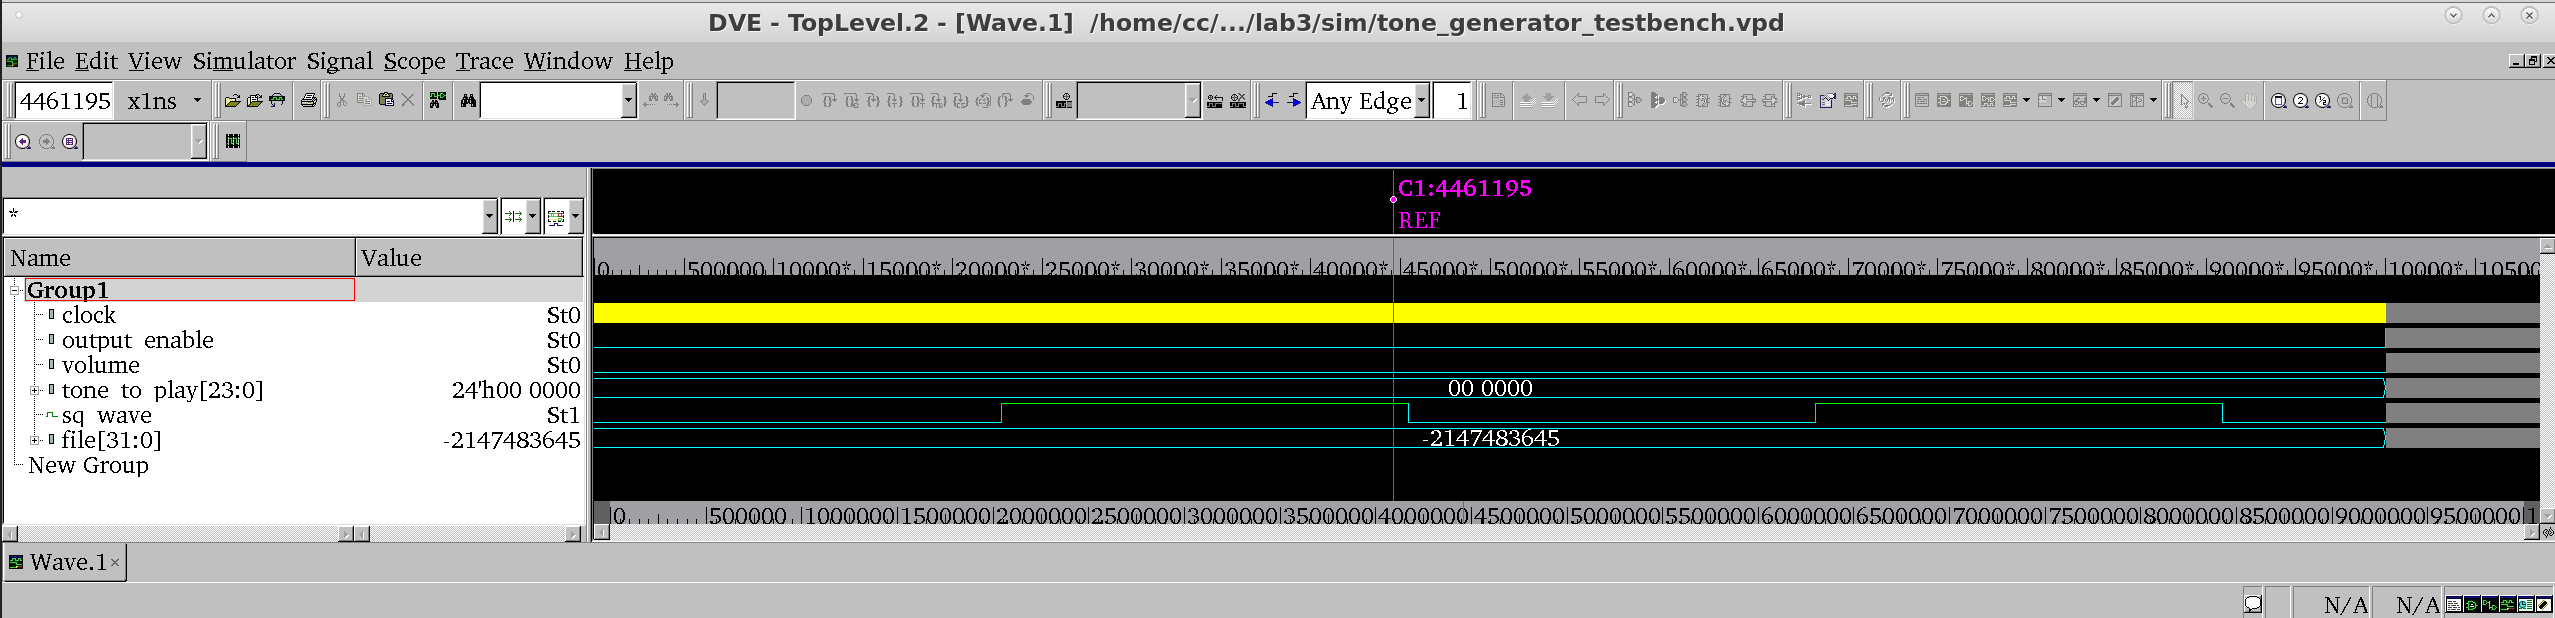
\includegraphics[width=\textwidth]{figs/dve_wave.png}
  \caption{DVE Waveform Viewer}
  \label{fig:dve_wave}
\end{figure}

Here are a few useful shortcuts:
\begin{itemize}
  \item \textbf{Click on waveform}: Sets cursor position
  \item \textbf{O}: Zoom out of waveform
  \item \textbf{+}: Zoom into waveform
  \item \textbf{F}: Fit entire waveform into viewer (zoom full)
  \item \textbf{Left Click + Drag Left/Right}: Zoom in on waveform section
\end{itemize}

%\subsubsection{XSIM}
%Vivado has an integrated simulator, \textbf{xsim}, that can run your Verilog testbench.
%You can run XSIM on your laptop.
\subsubsection{Icarus Verilog}
Icarus Verilog is available on the lab machines.
To install Icarus and gtkwave locally, refer to the appendix.

Run \verb|make sim/tone_generator_testbench.vcd| to launch a simulation with Icarus and to produce a vcd waveform file.
You can open the VCD with DVE as in the previous section, or use gtkwave locally.

\subsection{Analyzing the Simulation}
After opening the waveform, you should be able to see the clock oscillate at the frequency specified in the testbench.
You should also see the \verb|output_enable| signal start at 0 and then become 1 after 10 ms.
However, you may see that the \verb|sq_wave| signal is just a red line. What's going on?

\subsubsection{Fixing Unknown Signals}
Blue lines (written as `Z' in Verilog) in a waveform viewer indicate high-impedance (unconnected) signals.
We won't be using high-impedance signals in our designs, so blue lines or `Z' indicate something in our testbench or DUT isn't wired up properly.

Red lines (written as `X' in Verilog) in a waveform viewer indicate unknown signals.
At the start of simulation, all registers in your DUT contain unknown values (represented as `x').
Since we don't have an explicit reset signal for our circuit to bring the \verb|clock_counter| to a defined value, it may be unknown for the entire simulation.

Let's fix this. In the future we will use a reset signal, but for now let's use a simpler technique. In \verb|src/tone_generator.v| add an initial value to any registers in your design.
\begin{minted}{verilog}
// Original code:
reg counter;

// Change to:
reg counter = 0;
\end{minted}

This tells the simulator that the initial value for this register should be 0.
For this lab, when you add new registers in your \verb|tone_generator| or any other design module, you should instantiate them with their initial value in the same way.
\textbf{Do not set an initial value for a 'wire' type net; it will cause issues with synthesis, and may cause X's in simulation.}

Now run the simulation again.
\subsubsection{Helpful Tip: Reloading Waveforms}
When you re-run your simulation and you want to plot the newly generated signals in DVE or gtkwave, you don't need to close and reopen the waveform viewer.
Use \verb|Shift + Ctrl + R| in gtkwave or \verb|File| $\rightarrow$ \verb|Reload Databases| in DVE to reload the waveform file.

\subsubsection{Listen to Your Square Wave Output}
Look at the file written by the testbench at \verb|lab3/sim/output.txt|.
It contains a sequence of 1s and 0s that represent the output of your \verb|tone_generator| sampled at 44.1 kHz.
Use a Python script that can take this file and generate a \verb|.wav| file that you can listen to.

Go to the \verb|lab3/| directory and run the command:

\verb|python3 scripts/audio_from_sim.py sim/output.txt|

This will generate a file called \verb|output.wav|. Run this command to play it:

\verb|play output.wav|

If \verb|play| doesn't work, try running \verb|aplay output.wav|.
You should hear a 220Hz square wave. Compare it with a \href{https://www.szynalski.com/tone-generator/}{reference tone generator}.

\section{Top-Level Wiring and Tone Generator on the FPGA}
Open \verb|src/z1top.v| and instantiate the \verb|tone_generator|.
Connect \verb|square_wave_out| to \verb|aud_pwm|.
Drive the unused inputs of the \verb|tone_generator| to 0.
Set \verb|aud_sd| to 1 to enable the audio output.

\subsection{Make-Based FPGA Flow}
We're no longer using the Vivado GUI to run the FPGA flow, but a Makefile driven flow instead.
Inside \verb|lab3| you can run the following:
\begin{itemize}
  \item \verb|make lint| - Lint your Verilog with Verilator; checks for common Verilog typos, mistakes, and syntax errors
  \item \verb|make synth| - Synthesize \verb|z1top| and put logs and outputs in \verb|build/synth|
  \item \verb|make impl| - Implement (place and route) the design, generate the bitstream, and put logs and outputs in \verb|build/impl|
  \item \verb|make program| - Program the FPGA with the bitstream in \verb|build/impl|
  \item \verb|make vivado| - Launch the Vivado GUI
\end{itemize}

You should start with \verb|make synth|, and check the log in \texttt{build/synth/synth.log} for any warnings or errors.
Then build a bitstream by running \verb|make impl|.
Program the FPGA by running \texttt{make program}.

\textit{Warning:} the audio output will be loud, don't put your headphones near your ear.
Plug in headphones and make sure you hear a buzzing noise at 220Hz.
Again, compare the tone to a \href{https://www.szynalski.com/tone-generator/}{reference tone generator}.
To stop the buzzing, you can press the \verb|SRST| button on the top-right of the Pynq.

\section{Enhancements}
\subsection{Switching the Wave On and Off}
Now you have a tone, but it can't be toggled on and off without pulling the power to the FPGA board or resetting it.
Let's use the \verb|output_enable| input of the \verb|tone_generator| module to gate the square wave output.
When \verb|output_enable| is 0, you should pass 0 to the \verb|square_wave_out| output, but when \verb|output_enable| is 1, you should pass your square wave to \verb|square_wave_out|.

Wire up the \verb|output_enable| signal to the first slide switch (\verb|SWITCHES[0]|) in \verb|z1top|.

Run the design flow and program the board. You should now hear a buzzing noise at 220Hz that can be turned on or off by toggling the first slide switch.

\subsection{System-Level Testbench}
We previously tested the \verb|tone_generator| on its own as a unit-test.
We can also test the top-level module \verb|z1top| which contains the \verb|tone_generator|.
An example testbench is in \verb|sim/z1top_testbench.v|.
Run the system-level testbench with: \verb|make sim/z1top_testbench.vpd|.

Play around with the testbench by altering the clock frequency, changing when you turn on \verb|output_enable| and verifying that you get the audio you expect.

\begin{texexptitled}{Testbench Observations}{}
  \begin{enumerate}[a)]
    \item If you increase the clock frequency from 125 Mhz, would you expect the tones generated by your \verb|tone_generator| to be of a higher or lower frequency than was generated with the 125 MHz clock? Why?
    \item Prove that the \verb|output_enable| input of your \verb|tone_generator| actually works in system-level simulation. Take a screenshot.
  \end{enumerate}
\end{texexptitled}

\subsection{Volume Adjustment}
The tone from the FPGA is too loud!
To fix this, when the square wave is high, do not emit a continuous 1 on the \verb|square_wave_out| port, but instead emit a PWM waveform with a duty cycle selected by the \verb|volume| input.
\begin{itemize}
  \item \verb|volume = 1| $\rightarrow$ duty cycle = 50\% when square wave is high
  \item \verb|volume = 0| $\rightarrow$ duty cycle = 25\% when square wave is high
\end{itemize}

\begin{texexptitled}{Verify Volume Adjustment}{}
  \begin{enumerate}[a)]
    \item Modify the system-level testbench to iterate through both \verb|volume| settings. What changes were made?
    \item Take a screenshot of the waveform showing how \verb|square_wave_out| is PWMed for each \verb|volume| setting.
  \end{enumerate}
\end{texexptitled}

Wire up the \verb|volume| signal to the second slide switch (\verb|SWITCHES[1]|) in \verb|z1top|.
Create a bitstream and test the volume configuration on the FPGA.

\subsection{Configurable Frequency tone\_generator}
Let's extend our \verb|tone_generator| so that it can play different notes.
There is a 24-bit input to the \verb|tone_generator| called \verb|tone_switch_period|.

The \verb|tone_switch_period| describes how many cycles of the \verb|clk| should pass before the square wave output is toggled.
For example a \verb|tone_switch_period| of 150000 tells us to invert the square wave output every 150000 clock cycles, which for a 125 Mhz clock translates to a $\sim 417$ Hz square wave. Here is the derivation:

\begin{align*}
  \frac{2 \cdot 150000 \text{ cycles}}{1 \text{ second}} &= \frac{125 \times 10^6 \text{ cycles}}{1 \text{ second}} \div \frac{f \text{ cycles}}{1 \text{ second}} \\
  f &\approx 417 \text{ Hz}
\end{align*}

Note we multiply the \verb|tone_switch_period| by 2 to get the actual period of the square wave.

You should invert the square wave output every \verb|tone_switch_period| cycles.
Remember to initialize any new registers declared in your \verb|tone_generator| to their desired initial value to prevent unknowns during simulation.

You should also handle the case when \verb|tone_switch_period| is 0.  In this case disable the tone output.

\begin{texexptitled}{Verify Configurable Frequency}{}
  \begin{enumerate}[a)]
    \item Create a testbench that plays some simple melody that you define. Save the audio file for checkoff.
    \item Verify that when \verb|tone_switch_period| is set to 0, the \verb|square_wave_out| output doesn't toggle. Attach a screenshot.
  \end{enumerate}
\end{texexptitled}

\subsubsection{Try the Configurable Frequency tone\_generator on the FPGA}
Modify \verb|z1top.v| to wire \verb|tone_switch_period| to \verb|BUTTONS[3:0]|
input to the \verb|tone_generator|. You should tie the \verb|tone_switch_period| to \verb|BUTTONS[3:0]|, left-shifted by 16 bits (effectively a multiplication by 65536).
This will allow you to control the \verb|tone_switch_period| from 65536 to 983040.
Leave \verb|SWITCHES[0]| to control \verb|output_enable| and \verb|SWITCHES[1]| to control \verb|volume|.

\begin{minted}[tabsize=4]{verilog}
    tone_generator audio_controller (
        .output_enable(SWITCHES[0]),
        .volume(SWITCHES[1]),
        .tone_switch_period(BUTTONS[3:0] << 16),
    );
\end{minted}

Run the usual flow to put your new \verb|tone_generator| on the FPGA.
Verify that pushing the buttons changes the frequency of your \verb|tone_generator|.

\section{Checkoff}
In any lab session, show the TA the following:
\begin{enumerate}
  \item Show the RTL you used to create your tone generator
  \item Play an audio file that demonstrates playing a melody using the tone generator
  \item Demonstrate your tone generator on the FPGA
    \begin{enumerate}
      \item Demonstrate muting the output with a switch
      \item Demonstrate the volume control
      \item Demonstrate the runtime frequency configurability with the buttons
    \end{enumerate}
\end{enumerate}

Submit a lab report with answers and screenshots for the questions in this lab to Gradescope.

\appendix
\section{Local Dev Setup}
We aim for the labs to be do-able using your laptop connected to a Pynq board.
Refer to the Lab 2 spec's appendix to install Vivado locally.

The other dependencies for this lab are \verb|make|, \verb|iverilog|, and \verb|gtkwave|.
We'll cover installing them for each OS.

\subsection{Linux/OSX}
\begin{enumerate}
  \item Add vivado to your \verb|$PATH| by adding this in your \verb|.bashrc|:

    \verb|export PATH="/opt/Xilinx/Vivado/2019.1/bin:$PATH"|
  \item Install Icarus Verilog
    \begin{itemize}
      \item Linux: \verb|sudo apt install iverilog|
      \item OSX: \verb|brew install icarus-verilog|
    \end{itemize}

  \item Install gtkwave
    \begin{itemize}
      \item Linux: \verb|sudo apt install gtkwave|
      \item OSX: \href{https://sourceforge.net/projects/gtkwave/files/gtkwave-3.3.100-osx-app/gtkwave.zip/download}{Download the app}
    \end{itemize}
\end{enumerate}

In a terminal you should be able to successfully run \verb|vivado|, \verb|iverilog|, \verb|gtkwave|.

\subsubsection{Sharing Pynq USB Device from OSX to Linux VM}
\subsection{Windows}
\textbf{TODO} add vivado bin to PATH, how to run tests, how to view waves with gtkwave

Installing Icarus locally on OSX or Linux is as easy as:
\begin{minted}{bash}
  apt install iverilog
  brew install icarus-verilog
\end{minted}

Windows packages for \href{http://bleyer.org/icarus/}{Icarus are available}.

\section*{Ackowlegement}
This lab is the result of the work of many EECS151/251 GSIs over the years including:
\begin{itemize}
\item Sp12: James Parker, Daiwei Li, Shaoyi Cheng
\item Sp13: Shaoyi Cheng, Vincent Lee
\item Fa14: Simon Scott, Ian Juch
\item Fa15: James Martin
\item Fa16: Vighnesh Iyer
\item Fa17: George Alexandrov, Vighnesh Iyer, Nathan Narevsky
\item Sp18: Arya Reais-Parsi, Taehwan Kim
\item Fa18: Ali Moin, George Alexandrov, Andy Zhou
\end{itemize}

\end{document}
